\documentclass[a4paper]{article}



%% Language and font encodings
\usepackage[english]{babel}
\usepackage[utf8x]{inputenc}
\usepackage[T1]{fontenc}
\usepackage[compat=1.0.0]{tikz-feynman}
\usepackage{listings}


%% Sets page size and margins
\usepackage[a4paper,top=3cm,bottom=2cm,left=3cm,right=3cm,marginparwidth=1.75cm]{geometry}

%% Useful packages
\usepackage{amsfonts}
\usepackage{amsmath}
\usepackage{graphicx}
\graphicspath{ {./img/} }
\usepackage[colorlinks=true, allcolors=blue]{hyperref}
\usepackage{float}
\usepackage{enumerate}
\usepackage{subfig}

\title{REYES Nuclear Physics Mentoring Week 5}
\author{Aman Kumar}

\begin{document}
\maketitle
\section{Introduction}
In Week 5 we began our discussion with the scattering theory and Feynman Diagrams. For the first example, we discussed the collison of two
particles having mass $m$ and momentum $\vec{p}$ and $-\vec{p}$ respectively. When they collide the following situations can happen: 
\begin{enumerate}
    \item $E$ : Total Energy of the system is between $2m$ and $3m$ : \emph{Production of two particles with same mass going in opposite directions with same momentum.}
    \item $E > 3m$ : \emph{Production of 3 or more particles moving in different directions.}
\end{enumerate}

The second case is the one that Quantum Mechanics fails to describe. Here Quantum Field Theory (QFT) comes to rescue. The QFT describes the particles as excitations in 
their repective field. And their energy describes their mass. 
\\
Later we discussd about basics of QFT, begining with the basics like : What actually is a Field? Along wit the discussion on scalar and vector fields.

\section{Intro to Feynman Diagrams}
The introduction to Feynman Diagrams began with the discussion with the particles interacting or just propagating. More precisely, we discussed how a particle can 
either propagate freely with time or can interact with other particles (if available). \emph{The momentum and mass-energy is always conserved during interactions.}
\\
Our discussion then went towards the more complicated interactions like 2 particle productions, exchange of photons and then indistinguishable particles after interaction.
\subsubsection{Feynman Rules}
\begin{enumerate}
    \item Vertices = $-i\lambda$; where -ve sign is just a convention and $\lambda$ is a parameter. 
    \item For external legs in vertices you get a factor of $+1$
    \item For internal lines [propagtors] you get a factor of $\dfrac{i}{P^2 - M^2 + i\epsilon}$; \\with $P = E^2 - p_x^2 - p_y^2 -p_z^2$ and M = Mass of particle.$\epsilon$ is an intermediate parameter, but ultimately we use take it as zero.
    \item For intermediate unconfirmed momentums, we integrate $\int\dfrac{d^4k_1}{(2\pi)^4}$,$\int\dfrac{d^4k_2}{(2\pi)^4}$, etc.
    \item Divide by a symmetry factor = number of permutation of internal lines that leave the diagram unchanged!
\end{enumerate}
Using the above rules we can convert any feynman diagrams into mathematical equations. These rules give the contribution to the scattering amplitude.
\emph{The contributions are all multiplied.}

\section{Assignment}
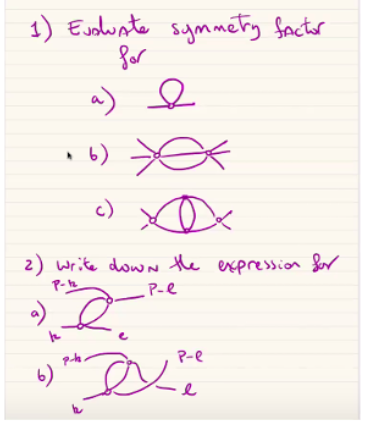
\includegraphics{assign}
\begin{enumerate}
    \item \begin{enumerate}
        \item Symmetry factor = 1 as there's no permutation.
        \item Symmetry fator = 3! = 6 (3 propagators which remain unchanged.)
        \item Symmetry factor = 2*2! = 4 (There are 2 pairs of unique propgators. Based on momentums, the interaction in middle is same so no permutation.) [Apply nodal analysis for momentum]
    \end{enumerate}
    \item \begin{enumerate}
        \item Equation = $\dfrac{(- i \lambda)^2}{1} \int\dfrac{d^4x}{(2 \pi)^4}(\dfrac{i}{x^2 - m^2 + i\epsilon})^2$ [Symmetry Factor = 1, discussed in 1(c)]
        \item Equation = $\dfrac{(- i \lambda)^2}{1}\int\dfrac{d^4x}{(2 \pi)^4}(\dfrac{i}{x^2 - m^2 + i\epsilon})^2$
    \end{enumerate}
\end{enumerate}


\end{document}